
    The issue of cooling the ambient air to process temperatures at around $90 K$ is not an easy
    one. The main hindrance is, that a heat sink at this temperature level is not readily available.
    Lucky thermodynamics offer a different way to reach such temperatures. In order to do so,
    the ambient air first needs to be compressed and then expanded again. Cooling then occurs
    by either exploiting the \emph{Joule-Thompson} effect or isentropic expansion. First a few
    comments are made about the compression stage, while afterwards the governing principles
    for cooling by expansion will be described.

    \subsubsection{Multi-stage compression}
        \begin{figure}
            \center
            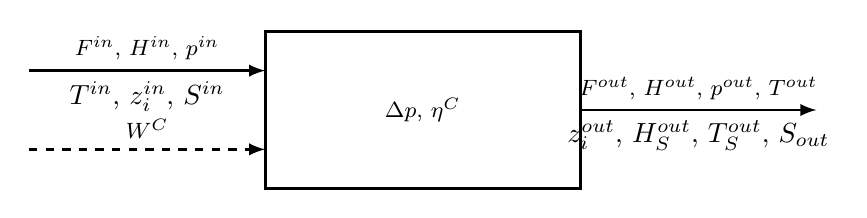
\begin{tikzpicture}[arrow/.style={line width=1pt,->,>=latex}]
	\draw [line width=1pt] (-2,2) rectangle (2,0) node at (0,1) {\footnotesize $\Delta p$, $\eta^C$};
	\draw [arrow] (-5,1.5) -- (-2,1.5) node [pos=0.5, above] {\footnotesize $F^{in}$, $H^{in}$, $p^{in}$} node [pos=0.5, below] {$T^{in}$, $z_i^{in}$, $S^{in}$};
	\draw [line width=1pt,->,>=latex,dashed] (-5,0.5) -- (-2,0.5) node [pos=0.5, above] {\footnotesize $W^C$};
	\draw [arrow] (2,1) -- (5,1) node [pos=0.5, above] {\footnotesize $F^{out}$, $H^{out}$, $p^{out}$, $T^{out}$} node [pos=0.5, below] {$z_i^{out}$, $H_S^{out}$, $T_S^{out}$, $S_{out}$};
\end{tikzpicture}�
            \caption{Multi-stage compression.}
            \label{fig:multi_stage_compression}
        \end{figure}

        Compressors and expanders are among the most common process equipment. A multitude of processes
        utilizes them as primary or auxiliary units. In the context of cryogenic air separation the
        compression plays a major role, as it enables to reach temperatures needed for liquefying
        air and gases in general. As the compression of gases is always associated with a significant
        reduction in volume it requires large amounts of energy. Thus in addition to significantly
        contributing to the capital cost of the process the compression stage is responsible for
        the majority of the operating cost encountered in the ASU process.

        The rigorous modeling of continuous flow machines in terms of unit operations poses great challenges.
        For specific units it may be undertaken by means of CFD simulations or employing characteristics diagrams,
        which require extensive experiments or can be obtained from the manufacturer.
        For the purposes of process design however a simpler approach with unit efficiencies is appropriate.

        As a significant temperature increase goes along with the compression of air and in order to reduce
        the energy demand of the compression in general, it is beneficial, to use a multi stage compressor with
        inter-cooling stages as depicted in \figref{fig:multi_stage_compression}. This yields a lower energy consumption
        as a single stage unit for the same compression ratio.

        Subsequently the working equations for the compressor model used in the scope of this thesis are
        briefly summarized.

        A trivial material and component balance around the compressor yields the outlet molar flow-rate $F^{out}$
        as well as the outlet overall composition $z^{out}$
    	\Eq{eq:comp:MassBalance}{
    		0 = F^{in} - F^{out},
    	}%
    	\Eq{eq:comp:CompBalance}{
    		0 = z_i^{in} - z_i^{out} \eqannc.
    	}%
    	To calculate the mechanical work associated with the desired compression,
        first the isentropic case
    	\Eq{eq:comp:SInOut}{
    		S^{in} = S^{out}
    	}%
        is considered. With that the isentropic work $W_S$ is calculated. Here the exit enthalpy in the 
        isentropic case $H_S^{out}$ is used. 
    	\Eq{eq:comp:IsentropicWork}{
    		W_S = F^{in} \cdot (H^{in} - H_S^{out})
    	}%
        With the isentropic efficiency $\eta^C$, the actual work $W$ and outlet enthalpy determined, 
    	\Eq{eq:comp:WEta}{
    		W \cdot \eta^C = W_S, 
            W_S = F^{in} \cdot (H^{in} - H^{out}). 
    	}%
        Finally the pressure drop over the unit needs to be considered
    	\Eq{eq:comp:PressureDrop}{
    		p^{out} = p^{in} + \Delta p. 
    	}%

    \subsubsection{Cooling by expansion}
        The liquefaction of gases requires temperatures well below ambient conditions. In order to attain
        such conditions one cannot utilize natural occurring coolants as they are not available at the required
        temperature level. Rather cooling effects that can occur during the expansion of gases are exploited.
        First we consider the expansion through an expansion valve or so called \emph{Joule-Thompson} - valve.
        In an rather accurate approximation, expansion through a valve can approximated as an isenthalpic
        process ($h_1 = h_2$). To describe the change in temperature during isenthalpic expansion
        the \emph{Joule-Thompson} coefficient
        \Eq{}{
            \mu_{JT} = \left(\fracddpart{T}{p}\right)_h,
        }
        which denotes pressure derivative of the temperature at constant enthalpy can be considered.
        This can be transformed into
        \Eq{}{
            \mu_{JT} = \frac{1}{c_p} \left[T \left(\fracddpart{v}{T}\right)_p - v \right]
        }
        \ncg{\mu_{JT}}{\emph{Joule-Thompson} coeffivcient}{\frac{K}{Pa}}

        \begin{figure}
            \center
            \input{GNUPlot/pr_isenthalpes}
            \caption{Isenthalpes computed by Peng-Robinson EOS.}
            \label{fig:pr_isenthalpes}
        \end{figure}
%        \stdfig{GNUPlot/pr_isenthalpes}{Isenthalpes computed by Peng-Robinson model.}{fig:pr_isenthalpes}{}

        If we employ the Peng-Robinson equation of state, which is appropriate for this mildly non-ideal system
        \cite{AndreasPfennig.2003}, we can plot the isenthalpes for ambient air ($x_{N_2}=0.7812$, $x_{O_2}=0.2095$,
        $x_{Ar}=0.0093$ ) in a PT-diagramm (\figref{fig:pr_isenthalpes}).
        There we can see, that in certain ranges a decrease in pressure at constant enthalpy will result
        in an increase in temperature, while for other regions temperature decreases. It is interesting
        to mention that the non-idealities of a given gas give rise to this effect. For an ideal gas the
        temperature change at isenthalpic expansion would always be zero. Luckily for the cryogenic engineer
        real gases deviate from ideal behaviour especially at elevated pressures and low temperatures \cite{Barron.1985}.
        It is therefore important to give some consideration to the thermodynamic model used to describe the properties
        of the system in question, as the non-ideal properties need to be captured appropriately.

        A different way of expanding a compressed gas, is by letting it produce work in an fluid kinetic machine.
        If one assumes an adiabatic devices and disregards irreversible effects, this process can be viewed as
        isentropic. Analogous to the isenthalpic case an isentropic expansion coefficient can be defined
        \Eq{}{
            \mu_S = \left( \fracddpart{T}{p} \right)_S = \frac{T}{c_p} \left( \fracddpart{v}{T} \right)_p.
        }%
        \ncg{\mu_S}{isentropic expansion coefficient}{\frac{K}{Pa}}

        Here the derivative in the second form corresponds to the volumetric coefficient of thermal expansion
        $\beta$, which is always positive for gases, which in turn means, that an isentropic expansion
        will always result in an temperature decrease, whereas the isenthalpic expansion only led to a decrease for
        specific conditions. Furthermore an isentropic expansion over the same pressure range will always result in
        lower temperatures than an isenthalpic expansion. The reason that isentropic valves are most commonly used
        in liquefaction systems, is that those work producing machines cannot handle significant phase changes,
        which is after all the desired result of liquefaction.

        Traditionally only the isenthalpic expansion had been used within the cryogenic air separation process,
        since -- as mentioned before -- the air needs to be liquefied in order to be fed into be distilled. However
        in modern process configurations the isentropic expansion is also considered to recover some of energy
        form the compression.
